\section{Tank Drain Simulation using Finite-Differences}
This section examines how to simulate the time to drain a tank.  
This particular example is a common exercise in fluid mechanics and hydraulic engineering courses to motivate the concept of control volumes and the conservation of mass.  
The equations of motion are usually given (as they are here) based on an assumption of negligible energy loss as the tank drains\footnote{Bernoulli's equation.}.

The purpose is to gain some practice with numerical modeling techniques before trying more complex methods in hydraulics.
\subsection{Problem Description}
Consider the tank depicted in Figure \ref{fig:time2drain.pdf}.  The water depth in the tank at any instant is $z(t)$.  The tank cross-section area is $A_{tank}$ and the outlet cross section area is $A_{out}$.   The product of $A_{tank}$ and $z(t)$ is the volume in storage in the tank at some instant, and the outflow from the tank is $Q(t)$.
\begin{figure}[h!] %  figure placement: here, top, bottom, or page
   \centering
   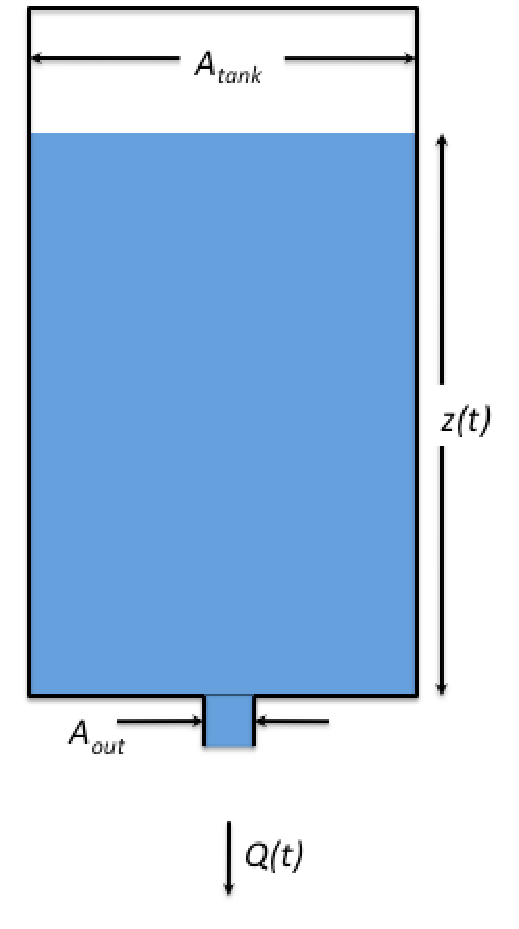
\includegraphics[width=3in]{./4-TankDrain/time2drain.pdf} 
   \caption{Storage tank with drain on bottom.}
   \label{fig:time2drain.pdf}
\end{figure}


As a first model consider the computation of 
\begin{enumerate}
\item Time to drain the tank from a known initial depth.
\item Storage in the tank at some given time.
\item Depth in tank at some given time.
\item Discharge rate at some instant in time.
\item How long to drain the tank to $\frac{1}{2}$ or $\frac{1}{4}$ full.
\end{enumerate}

All these questions are reasonable kinds of questions that could arise in some engineering design situation or (more likely) in an operations scenario. In this example the tank has constant cross section, but it is not a far stretch to imagine that the tank could represent a reservoir of variable geometry.  A practical reason to ask such questions arises in storm-water detention pond design (as well as reactor design in wastewater when dynamic flows are considered) --- the time to drain impacts the remaining capacity in a detention pond, the remaining capacity is what provides some measure of control for back-to-back storms.  If the tank drains too slowly, there will not be enough reserve for a back-to-back storm, whereas if the tank drains too fast it is hydraulically irrelevant.

While this problem seems detached from an open channel flow course, it [the problem] is not.  Each node in the open channel equations where flow depth is computed is essentially such a tank.  The tank area is not constant (instead the area is related to depth and reach distance), but like this tank the inflows and outflows are, in-part, governed by the depth already in the tank.


\subsection{Computational Approach}
This example will be handled first analytically (because it is simple to do so), then by a simple finite-difference scheme implemented in \textbf{R}

\subsection{Problem Analysis --- Development of the Analytical Solution}
To write an equation or set of equations for this problem, the relationship of tank depth, areas, and discharges must be specified.

If we write Bernoulli's equation along a streamline in the tank from the free surface to the outlet we would arrive at something like
\begin{equation}
\frac{p_{fs}}{\gamma}+\frac{V_{fs}^2}{2g}+z_{fs} = \frac{p_{out}}{\gamma}+\frac{V_{out}^2}{2g}+z_{out}
\label{eqn:tank_bernoulli}
\end{equation}

If we invoke the following reasonable assumptions:
\begin{enumerate}
\item $p_{fs}~=~0$ Free surface at zero gage pressure.
\item $p_{out}~=~0$ Pressure in jet is $\approx~0$.
\item $V_{fs} << V_{out}$ Free surface velocity is small relative to the outlet velocity.
\item $z_{out}~=~0$ the outlet is the datum.
\end{enumerate}

The resulting relationship between depth, and discharge is
\begin{equation}
Q(t)=A_{out} \times \sqrt{2gz(t)}
\label{eqn:tank_discharge}
\end{equation}

Now we have an equation of motion.  A mass balance in the tank requires that the storage decrease as the tank drains. Thus relating the change in tank depth and discharge produces the ordinary differential equation (ODE) that governs (at least in our model world) the tank.

\begin{equation}
A_{out} \times \sqrt{2gz(t)}=-A_{tank} \times \frac{d z}{d t}
\label{eqn:tank_ode}
\end{equation}

If one collects the constants $\frac{-A_{out}}{A_{tank}}\sqrt{2g} = \alpha$ the ODE is a little simpler to examine\footnote{The constants can be collected in this case because the geometry stays constant in the tank --- changing geometries would have areas as functions of depth and could not be collected in this fashion.}

\begin{equation}
\alpha  [z(t)]^{\frac{1}{2}}=  \frac{d z}{d t}
\label{eqn:tank_characteristic_ode}
\end{equation}

Equation \ref{eqn:tank_characteristic_ode} can be separated and integrated

\begin{equation}
\int_0^T{\alpha~dt }= \int_{z(0)}^0{ \frac{d z}{ [z(t)]^{\frac{1}{2}}} }
\label{eqn:tank_characteristic_integrated}
\end{equation}

The solution is

\begin{equation}
z(t)=(z(0)^{\frac{1}{2}}-\frac{\alpha}{2}t)^2
\label{eqn:tank_characteristic_solution}
\end{equation}

\subsubsection{Application of Analytical Solution in \textbf{R}}
This section presents the analytical solution coded in Excel, \textbf{R}, and \texttt{FORTRAN}.  


Analytical solutions are usually straightforward to represent in environments like \textbf{R}.  In this example, a single line of code builds the relationship and a couple more lines for a plot.

\begin{verbatim}
> depth<-function(alpha,time,initialDepth){(sqrt(initialDepth)-0.5*alpha*time)^2}
> tt<-seq(1,1000)
> plot(tt,depth(alpha,tt,5),xlab="Time (minutes)",ylab="Depth (meters)")
\end{verbatim}

The actual ``plot'' is left as an exercise. 

\subsection{Problem Analysis --- Development of the Finite-Difference Approximation}
The finite difference approximation follows the same principles up to Equation \ref{eqn:tank_characteristic_ode} then approximates the derivative term by its difference quotient for small time steps\footnote{Recall the fundamental theorem of calculus where the difference quotient is taken to the limit and this limit is called the derivative --- here we don't go to the limit, instead using small but finite steps.}

\begin{equation}
\alpha  [z(t)]^{\frac{1}{2}}\approx~  \frac{\Delta z}{\Delta t}
\label{eqn:tank_characteristic_fda}
\end{equation}

Notice some features of \ref{eqn:tank_characteristic_fda}.  First the equal sign is changed to ``approximately'' equal; second the derivative is changed to a related rate.  The remainder of the ``equation'' is unchanged.  The trick here is to understand how to interpret the equation. 
\begin{quote}
The approximation states that the rate of change of depth with time is approximately equal to the product of the geometric and gravitational constant and the square root of the current depth. 
\end{quote}

Using this approximation, and knowing the depth in the tank to start produces an algorithm to explore the tank behavior.  First expand the difference equation.
\begin{equation}
\alpha  [z(t)]^{\frac{1}{2}}= \frac{z(t+\Delta t) - z(t) }{\Delta t}
\label{eqn:tank_expanded_fda}
\end{equation}

Then rearrange to isolate values at time $t+\Delta t$,

\begin{equation}
{z(t+\Delta t) } = z(t) + \Delta t \alpha  [z(t)]^{\frac{1}{2}}
\label{eqn:tank_update}
\end{equation}

All the terms on the right hand side are known and the equation\footnote{Now known as an update equation} tells the modeler how to approximate depth at a future time.  Because the analysis assumed the difference quotient is close to the derivative, the time steps need to be kept pretty small (in fact in many problems the time step is constrained by the physics for stability and by the computation regime for precision).

The particular update here is an implementation of Euler's method\footnote{One of many methods to approximate solutions to ordinary differential equations}.  There are other methods --- the reader should observe that the time difference scheme could be backwards so that the discharge could be at an unknown time, or a weighted average of the two times, or a variety of other ways to approximate the derivative.




\subsection{Application of the Finite-Difference Approximation in \textbf{R}}
This section presents the same set of ``solutions'' using the finite-difference model.  In these cases the underlying algorithm is that expressed by Equation \ref{eqn:tank_update}.

To model the tank using \textbf{R} the modeler needs to write the necessary equation structure in the proper order.  Listing \ref{lst:Time2Drain} is a crude implementation --- note how the update quotient is actually built with a test for near zero values to prevent attempted square root of a negative number.   
Also note how there is some flexibility to change the time step.

\begin{lstlisting}[caption=R code demonstrating time to drain calculations, label=lst:Time2Drain]
> # Time to Drain Model
> AreaTank<-987
> AreaPipe<-1
> alpha<-sqrt(2*9.8)*AreaPipe/AreaTank
> z<-numeric(0)  # define the depth array
> z[1]<-5.0 # initial depth
> dt<-5.0 # time step size
> # program the update difference quotient
> dzdt<-function(alpha,depth){if(depth >= 0.001)alpha*sqrt(depth) else 0}
> # update many times
> for (i in 1:500){z[i+1]=z[i]-dt*dzdt(alpha,z[i])}
> length(z) # get length for plotting
[1] 501
> time<-seq(0,500)*dt
> plot(time,z,xlab="Time (minutes)",ylab="Depth (meters)")
\end{lstlisting}  

The result of the plot call is displayed in Figure \ref{fig:Time2DrainR.pdf}

\begin{figure}[htbp] %  figure placement: here, top, bottom, or page
   \centering
   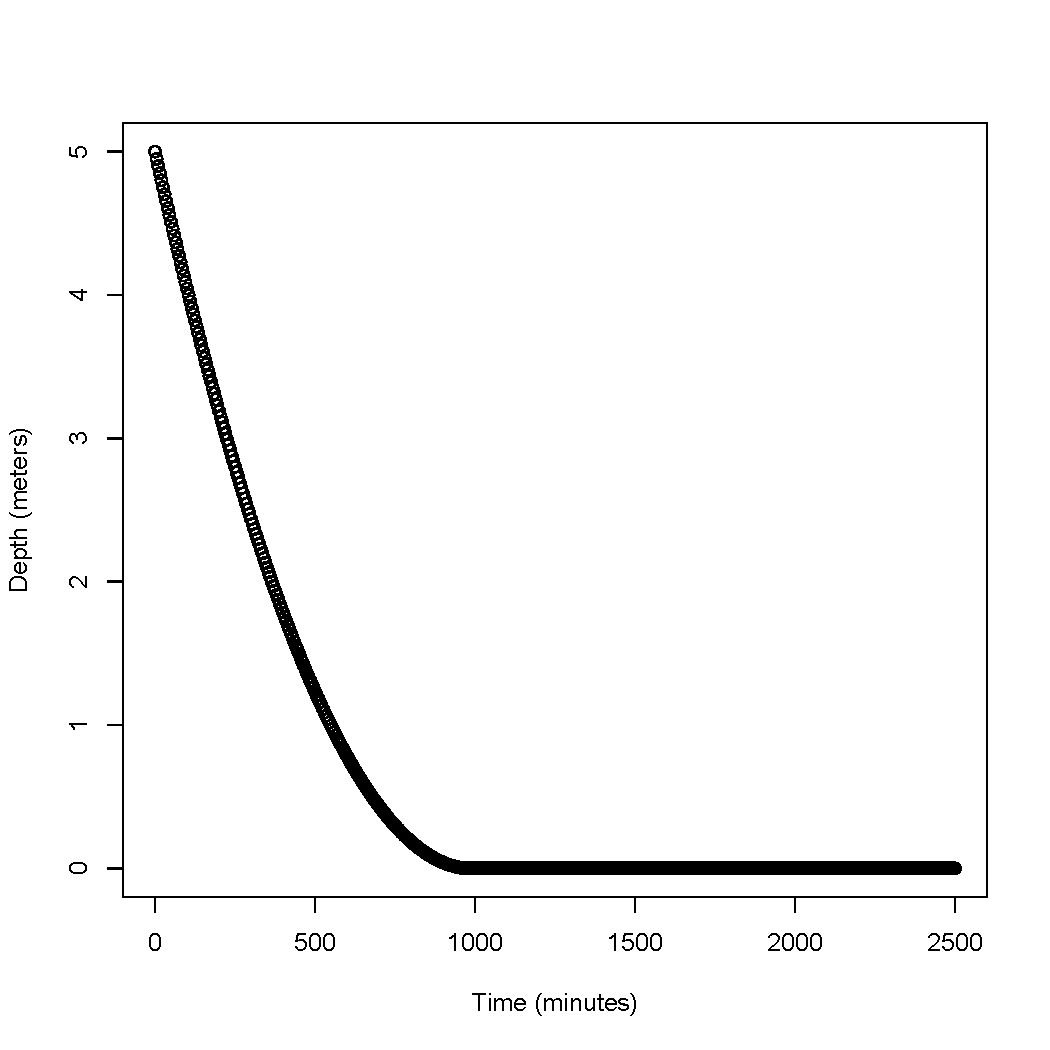
\includegraphics[width=5in]{./4-TankDrain/Time2DrainR.pdf} 
   \caption{Plot of relationship of elapsed time and depth of water in tank.}
   \label{fig:Time2DrainR.pdf}
\end{figure}

The plot displays a lot of zero values, the student should explore tricks to plot only the interesting portion of the behavior.  The student should also explore how to plot both the analytical and numerical solution on the same graph.

What this section presented is actually quite simple.  The engineer in any case will have to conceptualize the physical system into a structure amenable to mathematical representation.  The tools are the conservation of mass, momentum, and energy.  Then relationships between components must be established --- generally time, lengths, and forces are somehow related.  These relationships, whether empirical or fundamental constitute the basis to build a model to reality.

Next the modeler has to convert these relationships into a structure that can be solved using the tools at hand: in this case \textbf{R}.  Finally the application is built and used for the problem of interest.  While intellectually desirable to have a fairly general tool, the engineer should never be afraid to use a purpose built tool if a general tool is unavailable.  Be sure to test the tool and know its limitations.

In the example a simple hydraulics computation was presented to motivate these modeling steps.  
Solutions were constructed in the \textbf{R} programming environments.   

\subsection{Exercise Set 4}
\begin{enumerate}

\item Adapt the \textbf{R} script and build a simulator that approximates the depth of water in a cylindrical drum lying on its side as a function of time.  
Figure \ref{fig:drum} is a sketch of the drum of interest. 
Also desired is the volume in storage in the drum as a function of time.

\begin{figure}[h!] %  figure placement: here, top, bottom, or page
   \centering
   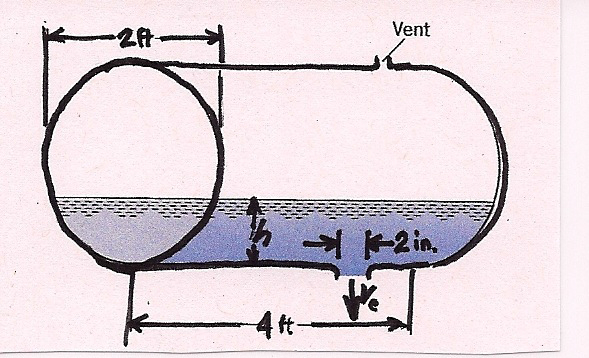
\includegraphics[width=4in]{./4-TankDrain/drum.jpg} 
   \caption{Sketch of drum dimensions}
   \label{fig:drum}
\end{figure}

The drum is drained by a 2-inch diameter short pipe at the bottom of the drum.  The velocity of water in the pipe is $V_e~=~\sqrt{2~g~h}$ where $g$ is gravitational acceleration and $h$ is water depth in the tank above the outlet.  The drum is 4-feet long and 2-feet in diameter.  Simulate the time to drain from $\frac{1}{2}$ full to empty, then generalize to any starting depth (up to the tank diameter).

Produce a time versus depth and time versus storage plot for the drum using \textbf{R}.  

Document your work in a short modeling report that includes conceptualization, problem analysis (development of requisite equations), coding, any testing, and finally the application of the model.  


\item Adapt the \textbf{R} script and build a simulator for a trough of arbitrary dimensions as shown in Figure \ref{fig:trough}.  

\begin{figure}[h!] %  figure placement: here, top, bottom, or page
   \centering
   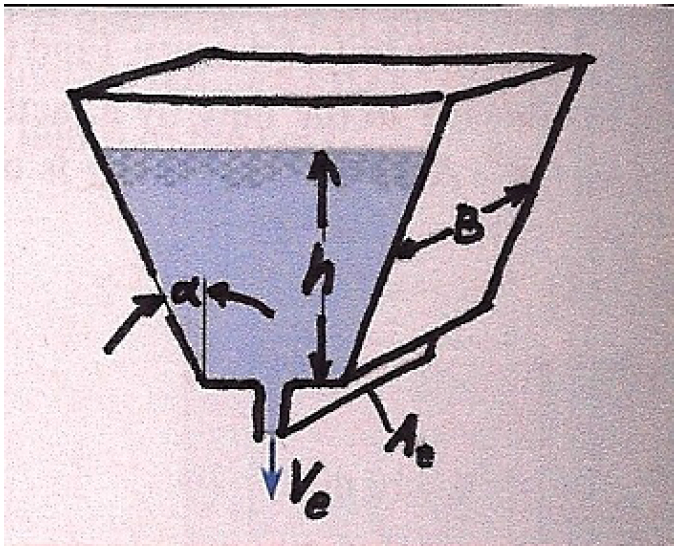
\includegraphics[width=4in]{./4-TankDrain/trough.jpg} 
   \caption{Sketch of trough dimensions}
   \label{fig:trough}
\end{figure}

The angle with the vertical of the sloping sides is $\alpha$, and the distance between the parallel ends is $B$.  
The width of the trough is $W_0 + 2h~tan~\alpha$, where $h$ is the distance from the trough bottom.  
The velocity of water issuing from the opening in the bottom of the trough is equal to $V_e~=~\sqrt{2~g~h}$.  
The area of the water stream at the bottom of the trough is $A_e$.  

Produce a drainage curve (time versus depth) for the case where $h_0~=~5m$, $W_0~=~1m$, $\alpha~=~30^o$, $B~=~10m$, and $A_e~=~1m^2$.

Document your work in a short modeling report that includes conceptualization, problem analysis (development of requisite equations), coding, any testing, and finally the application of the model.  
\end{enumerate}

These exercises are also located on the class server as \texttt{ES-4}.
%%%%%%%%%%%%%%%%%%%%%%%%%%%%%%%%%%%%%%%%%%%%%%%%%%%%%%%%